\chapter{Morphisms between Riemann surfaces}
\label{ch:morphism_riemann}

\section{Definition}

The definition is what we would expect --- since a Riemann surface's main feature is a
complex structure, a map $f \colon \CC \to \CC$ is a morphism between Riemann surfaces
if and only if it is holomorphic.

\begin{definition}
	\label{def:riemann_surface_morphism}
	Let $X$ and $Y$ be Riemann surfaces. A mapping $f \colon X \to Y$ is holomorphic at $p \in X$ if
	and only if there exists charts $\phi_1 \colon U_1 \to E_1$ on X with $p \in U_1$ and $\phi_2
	\colon U_2 \to E_2$ on $Y$ with $f(p) \in U_2$ such that the composition $\phi_2 \circ f \circ
	\phi_1\inv$ is holomorphic at $\phi_1(p)$. We say $f$ is a \vocab{morphism between Riemann
	surfaces} if and only if it is holomorphic at all points of $X$.
\end{definition}

In other words: $f$ is holomorphic if and only if it is holomorphic as function mapping
between local coordinates.

\begin{example}
	Some examples follows.
	\begin{itemize}
		\ii The function $f \colon \CC \to \CC$ by $f(x) = x^3$ is a morphism.

		Note that this function is not bijective. At each point $p \neq 0$, there is an open
		neighborhood on which $f$ has an inverse, but $f$ has no inverse at $0$.
		\ii The embedding of the complex plane into the Riemann sphere, $\CC \injto \CC_\infty$, is
		a morphism.
	\end{itemize}
\end{example}

\section{Functions to the Riemann sphere}
\prototype{The meromorphic function $\frac{1}{z}$ can be made into a holomorphic $\CC \to
\CC_\infty$ function.}

In this section, we will see that the Riemann sphere $\CC_\infty$ can be viewed as ``$\CC$ with a
point at infinity added''. This interpretation allows us to interpret meromorphic functions $f
\colon X \to \CC$ as holomorphic maps $g \colon X \to \CC_\infty$, which allows a much better
handling of meromorphic functions --- there's no longer any singularity, the resulting function
$g$ is holomorphic everywhere!

First, we see that $\CC_\infty$ can be naturally interpreted as $\CC$ with a single point added:
With notation as in \Cref{ex:riemann_sphere}, identify $\CC_\infty \setminus \{ N \}$ with $E_1$
(and thus with $\CC$) through the map $\phi_1$, and we let $\infty$ be the point $N$.

\begin{ques}
	Convince yourself that it makes sense to call the point $\infty$ --- for every sequence of
	points $\{ z_i \}$ on $\CC$ such that $|z_i| \to +\infty$, then $\phi_1\inv(z_i) \to \infty$
	on $\CC_\infty$ as a topological space.
\end{ques}

So, let $X$ be a Riemann surface, and $f \colon X \to \CC$ be a meromorphic function on $X$.
Naturally, $g$ can be defined by
\[ g(z) = \begin{cases}
	f(z) & \text{if }f(z) \neq \infty \\
	\infty & \text{if }f(z) = \infty.
\end{cases} \]
Then $g$ is continuous --- but furthermore, it's analytic.
\begin{ques}
	Clearly, at points $z \in X$ where $g(z) \neq \infty$, then $g$ is analytic.

	Convince yourself that $g$ is also analytic at $z \in X$ where $g(z) = \infty$.
	(With notation as in \Cref{ex:riemann_sphere},
	take a small open set $U \subseteq X$,
	and re-parametrize $g\im(U) \subseteq \CC_\infty$ by $t = 1/z$.)
\end{ques}

Therefore,
\begin{proposition}
	There is a one-to-one correspondence between meromorphic functions $f \colon X \to \CC$ and
	holomorphic maps $g \colon X \to \CC_\infty$ such that $g$ is not identically $\infty$.
\end{proposition}
Or, more informally,
\begin{moral}
	Plugging in the hole at $\infty$ of $\CC$ allows us to analytically extend meromorphic functions
	to $\CC \cup \infty$ maps which is holomorphic everywhere.
\end{moral}

\section{Some other nice properties}

We have just seen in the last section that the Riemann sphere $\CC_\infty$ allows us to remove the
singularities of a meromorphic functions.

Informally speaking, this is because $\CC_\infty$ is a ``compactfication'' of $\CC$ --- adding a
point to make it compact --- and compact Riemann surfaces enjoy many nice properties.

\begin{proposition}
	Let $X$ and $Y$ be compact, $f \colon X \to Y$ be holomorphic and not constant.
	For each point $y \in Y$, define $d_y$ be the total multiplicity of the points in the preimage
	of $y$.

	Then, $d_y$ is well-defined and constant.
\end{proposition}

You can see why this proposition is surprising:
\begin{example}[The proposition does not hold for smooth compact manifolds]
	Consider the following function $f \colon X \to Y$ between compact smooth real $1$-manifold,
	depicted as a plot with $x$ and $y$-axis.
	(Note that a compact $1$-manifold cannot be embedded into $\RR$, because compact subsets of
	$\RR$ are closed and bounded, thus necessarily have a boundary. A proper graph would live in a
	$4$-dimensional space, which is rather difficult to visualize, so we settle with an approximate
	representation.)

	\begin{center}
		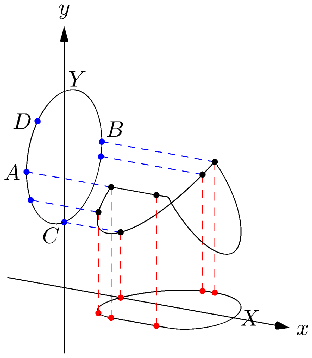
\includegraphics{3dfigures/pdf/morphism-scm-counterexample.pdf}
	\end{center}

	Here, $X$ and $Y$ are both isomorphic to the unit circle.

	We count the number of points in the fiber above each point in $Y$:
	\begin{itemize}
		\ii Above point $A$, there are infinitely many points.
		\ii Above point $B$, there is only one point. (You can argue that this point has
		``multiplicity $2$'' however)
		\ii Above point $C$, there are two points.
		\ii Above point $D$, the fiber is empty.
	\end{itemize}
\end{example}

\begin{definition}
	The value $d_y$ above is called the \vocab{degree} of the map $f$, written $\deg(f)$.
\end{definition}

\begin{example}
	The map $z \mapsto z^k$, when extended to a $\CC_\infty \to \CC_\infty$ map, has degree $k$.
\end{example}
If $t \neq 0$, then we know that $t$ has $k$ distinct $k$-th roots.
But if $t = 0$, its preimage only consist of the point $0$ --- in this case, we wish to say $z = 0$
is a ``multiple point'' --- we will formalize it next section when we defines the multiplicity of a
map.

If you have read \Cref{sec:homology_degrees},
this is in fact the same as the concept of a degree in homology when $X$ and $Y$ are both Riemann
spheres --- it counts how many spherical bags that $\img f$ consists of.
But, in this case, the theory is extra nice --- not only that the graph is homotopy equivalent to
one that covers each point $d$ times, but each point is in fact covered \emph{exactly} $d$ times!

This theme will be recurrent in complex analysis and Riemann surfaces. Basically:
\begin{moral}
	If the ``things'' are counted properly, the formula is very nice.
\end{moral}


The proof of the proposition is not difficult --- the main observation is that the theorem is true
for functions of the form $f(z) = z^n$, and locally around each point $p \in X$, $f$ is either an
isomorphism or has the form above.
So $d_y$ is locally constant, and thus constant because $Y$ is connected.


\section{Multiplicity of a map}
\prototype{$f(x) = (x-3)^2$ has $\mult_3(f) = 2$.}

In the previous section, we informally talk about the multiplicity of a map at a point. We will
rigorously define it in this section.

\begin{example}
	Consider the map $f \colon \CC \to \CC$ given by $f(z) = z^5 + 1$.

	Above each point $y \in \CC$, the fiber $f\pre(y)$ has $5$ points --- except when $y = 1$, then
	$f\pre(1) = \{ 0 \}$ has only 1 point.
\end{example}

This behavior is \emph{undesirable}, and we would like to say that the function $f$ maps $5$
``identical copies'' of the point $0$ to the point $1$.
(Another way you could see it is that, for each sequences $\{ y_i \}$ converging to $1$, there are
$5$ different sequences $\{ x_i \}$ converging to $0$ such that $f(x_i) = y_i$ for each $i$.)

Inspired by this, we will define multiplicity in a way such that:
\begin{itemize}
	\ii $z \mapsto z^m$ has multiplicity $m$, for integer $m \geq 1$.
	\ii If we perform an analytic reparametrization of the source or the target, then the degree
	does not change.
\end{itemize}
Turns out these two properties completely defines the degree! We have the following.
\begin{proposition}
	Let $f \colon X \to Y$ be a nonconstant holomorphic map defined at $p \in X$.
	Then there is a unique integer $m \geq 1$ such that, for every chart $\phi_2 \colon U_2 \to V_2$
	on $Y$ centered at $f(p)$ (that is, $\phi_2(f(p)) = 0$),
	there is a chart $\phi_1 \colon U_1 \to V_1$ on $X$ centered at $p$
	such that the induced map $\phi_2 \circ F \circ \phi_1\inv \colon V_1 \to V_2$
	has the form $z \mapsto z^m$.
\end{proposition}
In other words, once we fix a chart of $Y$, there exist a chart of (an open subset of) $X$
such that the induced map between open subsets of $\CC$ is a power map;
furthermore, the exponent is independent of the selection.
\begin{moral}
	Every map looks locally like $z \mapsto z^m$.
\end{moral}
\begin{proof}
	Essentially, use the Taylor expansion to determine $m$, then the selection of $\phi_1$ is pretty
	much fixed by the restrictions.
\end{proof}

\begin{definition}
	The value $m$ above is the \vocab{multiplicity} of $f$ at point $p$, written $\mult_p(f)$.
\end{definition}

\begin{example}[More examples of multiplicity of a map at a point]
	We consider some examples.
	\begin{itemize}
		\ii The function $z \mapsto z^{-2}$, extended to a $\CC \to \CC_\infty$ map,
		has multiplicity $2$ at point $0$ --- ``two copies'' of the point $0$ is mapped to the point
		$\infty$.
		\ii The function $f(z) = (z-1) (z-2)^5$ has $\mult_2(f) = 5$ --- more generally,
		if $p$ is a root of $f$, then $\mult_p(f)$ is the multiplicity of the root.
		\ii The function $z \mapsto z + 1$ has multiplicity $1$ everywhere --- in fact,
		the multiplicity of a nonconstant map at ``most'' points will be $1$.
	\end{itemize}
\end{example}

These are the official terms:
\begin{definition}
	A point $p$ such that $\mult_p(f) > 1$ is called a \vocab{ramification point}.
	In that case, the point $f(p)$ is called a \vocab{branch point}.
\end{definition}

\section{The sum of the orders of a meromorphic function}

Yet another case where we get a nice formula.
\begin{example}
	Let us consider some meromorphic $\CC_\infty \to \CC_\infty$ functions (defined by extending a
	$\CC \to \CC$ function the obvious way), and list the zeros and poles of it (with
	multiplicity).
	\begin{center}
	\begin{tabular}{ccc}
		Function & Zeros & Poles \\ \hline
		$5$ & None & None \\
		$(x+1)^2$ & $-1$, $-1$ & $\infty$, $\infty$ \\
		$\frac{1}{x^2+1}$ & $\infty$, $\infty$ & $i$, $-i$ \\
		$\frac{x+1}{x+2}$ & $-1$ & $-2$
	\end{tabular}
	\end{center}
\end{example}
Every time, the number of zeros equals the number of poles. This is not a coincidence!
\begin{proposition}
	Let $f \colon X \to \CC$ be a nonconstant meromorphic function on a compact Riemann surface $X$.
	Then \[\sum_p \ord_p(f) = 0. \]
\end{proposition}
Of course, we need $X$ to be compact --- there certainly are $\CC \to \CC$ functions that has
several zeros, but no poles.
\begin{proof}
	We extend $f$ to a $X \to \CC_\infty$ function, then the sum of multiplicities of points in the
	fiber of $0$ is equal to that in the fiber of $\infty$.
\end{proof}

\section{The Hurwitz formula}

\todo{write this one. It's quite nice actually}

\section{The identity theorem}

The following propositions are expected --- the same behavior is seen in complex analysis with
holomorphic functions.

\begin{theorem}
	Let $f, g \colon X \to Y$ be holomorphic maps between Riemann surfaces. If $f = g$ on a nonempty
	open subset of $X$, then $f = g$.
\end{theorem}
This is the analog of \Cref{prob:identity_thm}. Note that here the assumption that $X$ is connected
is used --- the disjoint union of two copies of $\CC$ is a smooth $2$-manifold, but not a Riemann
manifold.

That is,
\begin{moral}
	Holomorphic maps are \emph{rigid} --- the value of a function on a tiny subset determines its
	value everywhere.
\end{moral}
